% !TeX spellcheck = it_IT
\documentclass[12pt]{beamer}
\usetheme{default}

\usepackage[utf8]{inputenc}
\usepackage[italian]{babel}

\author{Gianguido Sorà}
\title{Linux in ambito smartphone e introduzione a SailfishOS}
%\subtitle{}
%\logo{}
\institute
{
  \medskip
    \textit{gianguidorama@gmail.com} 
}
\date{24 ottobre 2014}
%\subject{}
%\setbeamercovered{transparent}
%\setbeamertemplate{navigation symbols}{}

\begin{document}
\maketitle

\begin{frame}
\frametitle{Perché Linux?}
\begin{itemize}
\item Il kernel Linux è famoso per \textbf{scalabilità} ed \textbf{affidabilità}, oltre che per il suo modello di sviluppo.
\end{itemize}
\end{frame}

\begin{frame}
\frametitle{Perché Linux?}
\begin{itemize}
\item Il kernel Linux è famoso per \textbf{scalabilità} ed \textbf{affidabilità}, oltre che per il suo modello di sviluppo.
\item Adattarlo ai sistemi embedded è "semplice".
\end{itemize}
\end{frame}

\begin{frame}
\frametitle{Perché Linux?}
\begin{itemize}
\item Il kernel Linux è famoso per \textbf{scalabilità} ed \textbf{affidabilità}, oltre che per il suo modello di sviluppo.
\item Adattarlo ai sistemi embedded è "semplice".
\item Pur nascendo su Intel negli anni i port verso altre piattaforme sono stati molteplici, uno fra tutti quello verso \textbf{ARM}.
\end{itemize}
\end{frame}

\begin{frame}
\frametitle{Perché Linux?}
\begin{itemize}
\item Il kernel Linux è famoso per \textbf{scalabilità} ed \textbf{affidabilità}, oltre che per il suo modello di sviluppo.
\item Adattarlo ai sistemi embedded è "semplice".
\item Pur nascendo su Intel negli anni i port verso altre piattaforme sono stati molteplici, uno fra tutti quello verso \textbf{ARM}.
\item Reinventare la ruota \textbf{non} è una strada da percorrere.
\end{itemize}
\end{frame}

\begin{frame}
\frametitle{Linux su smartphone... ieri}
\begin{itemize}
\item Molte società multinazionali hanno \textit{provato} a sviluppare e vendere soluzioni mobile basate su Linux.
\end{itemize}
\end{frame}

\begin{frame}
\frametitle{Linux su smartphone... ieri}
\begin{figure}
\centering
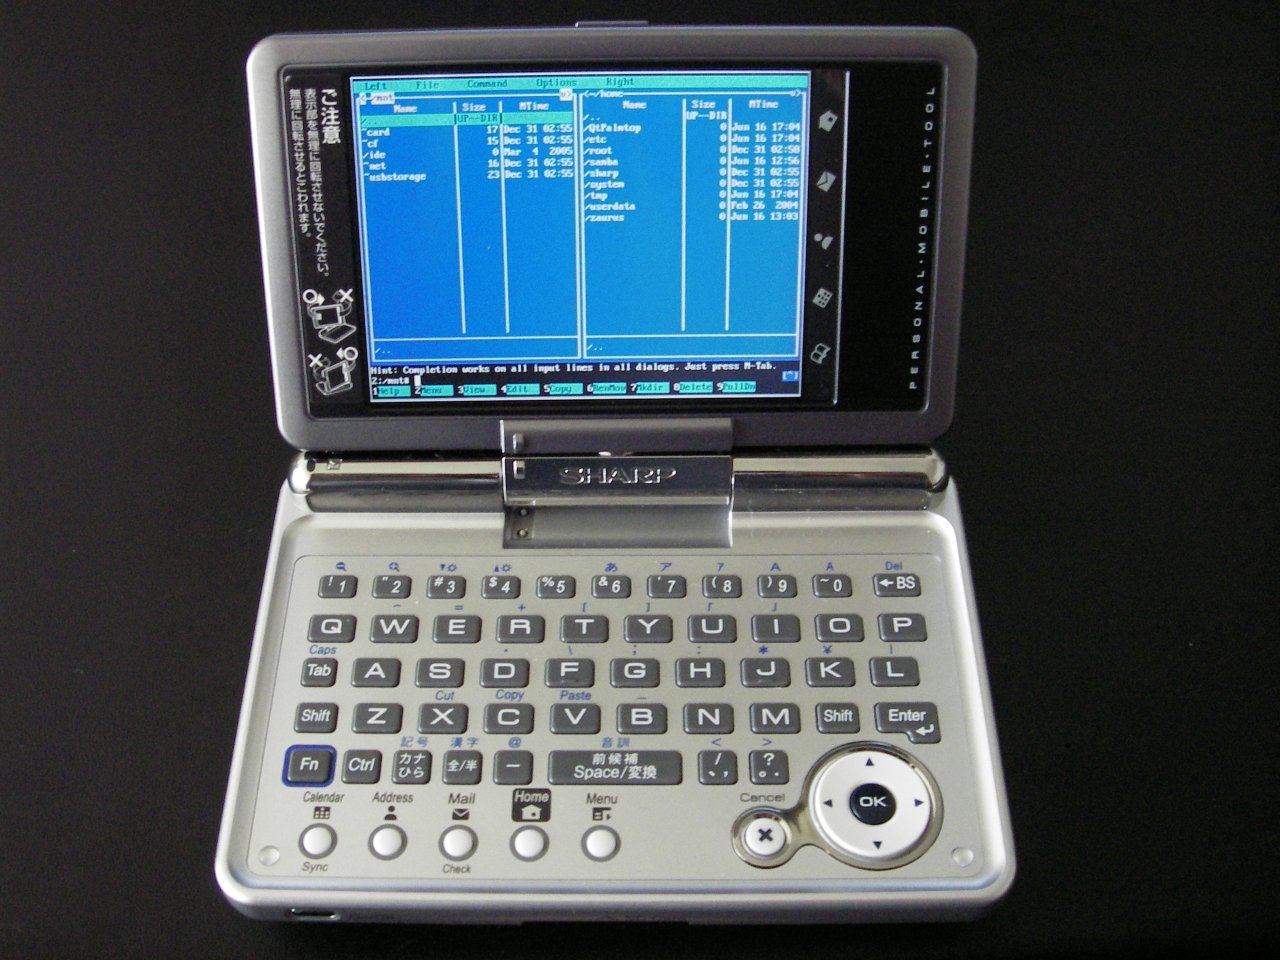
\includegraphics[width=0.7\linewidth]{/Users/Gianguido/Desktop/LinuxDayTalk/Sharp_Zaurus_SL-C1000_--_open_1280x960}
\caption[Sharp Zaurus]{Sharp Zaurus}
\label{Sharp Zaurus}
\end{figure}
\end{frame}

\begin{frame}
\frametitle{Linux su smartphone... ieri}
\begin{itemize}
\item Numerosi sono stati i progetti portati avanti dalla sola comunità Open Source che miravano alla creazione di un "unico\footnote{Hint: non hanno unificato nulla.} ambiente desktop mobile"
\end{itemize}
\end{frame}

\begin{frame}
\frametitle{Linux su smartphone... ieri}
\begin{figure}
\centering
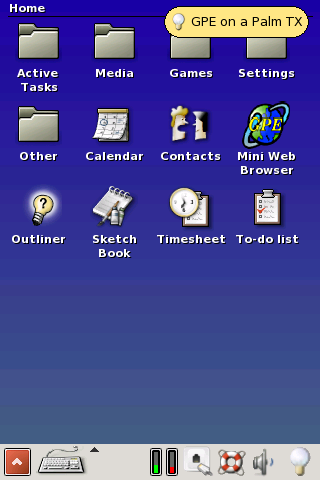
\includegraphics[scale=0.30]{/Users/Gianguido/Desktop/LinuxDayTalk/Gpe-palm-tx}
\caption[GPE]{GPE, basato sulle GTK+}
\label{fig:GPE}
\end{figure}
\end{frame}

\begin{frame}
\frametitle{Linux su smartphone... ieri}
\begin{figure}
\centering
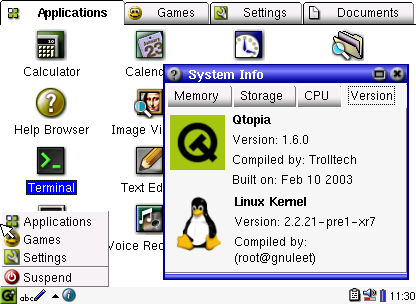
\includegraphics[width=0.7\linewidth]{/Users/Gianguido/Desktop/LinuxDayTalk/qtopia}
\caption[Qtopia]{Qtopia, basato sulle QT}
\label{fig:qtopia}
\end{figure}
\end{frame}

\begin{frame}
\frametitle{Linux su smartphone... ieri}
Purtroppo questi due progetti morirono, causa poca compatibilità hardware e poco interesse
\end{frame}

\begin{frame}
\frametitle{Linux su smartphone... "un po' meno ieri"}
\begin{itemize}
\item Grazie a Nokia ed al team di sviluppo kernel ARM Linaro, la situazione cambiò drasticamente
\end{itemize}
\end{frame}

\begin{frame}
\frametitle{Linux su smartphone... "un po' meno ieri"}
\begin{center}
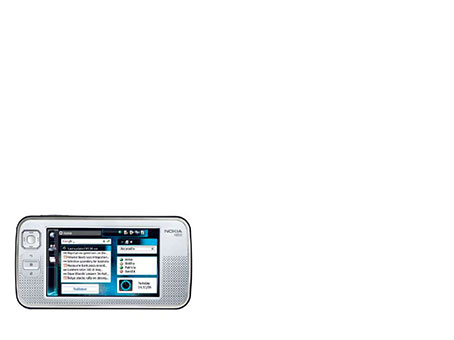
\includegraphics[width=0.7\linewidth]{/Users/Gianguido/Desktop/LinuxDayTalk/n1}
\end{center}
\end{frame}

\begin{frame}
\frametitle{Linux su smartphone... "un po' meno ieri"}
\begin{center}
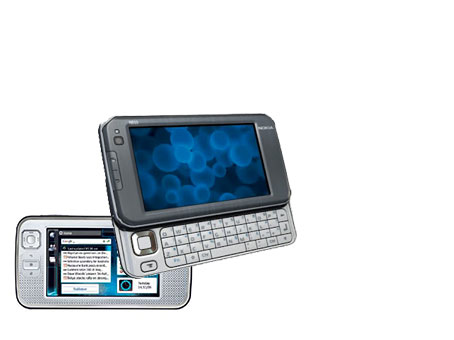
\includegraphics[width=0.7\linewidth]{/Users/Gianguido/Desktop/LinuxDayTalk/n2}
\end{center}		
\end{frame}

\begin{frame}
\frametitle{Linux su smartphone... "un po' meno ieri"}
\begin{center}
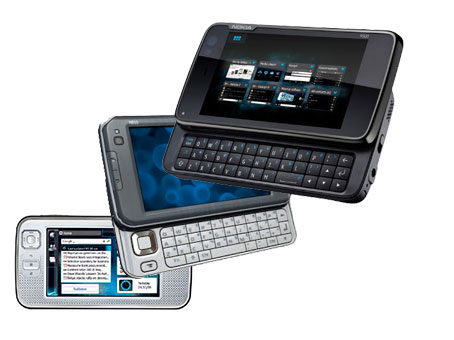
\includegraphics[width=0.7\linewidth]{/Users/Gianguido/Desktop/LinuxDayTalk/n3}
\end{center}			
\end{frame}

\begin{frame}
\frametitle{Linux su smartphone... "un po' meno ieri"}
\begin{center}
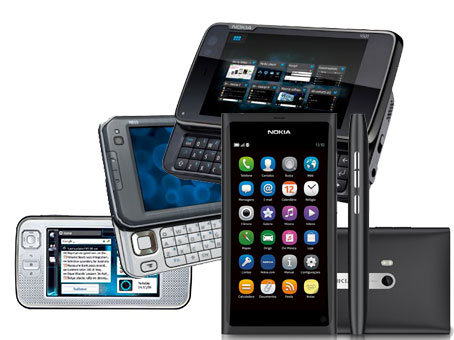
\includegraphics[width=0.7\linewidth]{/Users/Gianguido/Desktop/LinuxDayTalk/n4}
\end{center}				
\end{frame}

\begin{frame}
\frametitle{Linux su smartphone... "un po' meno ieri"}
\begin{itemize}
\item Altra protagonista indiscussa del panorama Linux mobile è Palm
\end{itemize}
\end{frame}

\begin{frame}
\frametitle{Linux su smartphone... "un po' meno ieri"}
\begin{itemize}
\item Altra protagonista indiscussa del panorama Linux mobile è Palm
\item I suoi smartphone \textbf{Pre} e \textbf{Pixi} hanno rappresentato il primo vero successo commerciale di Linux su smartphone.
\end{itemize}
\end{frame}

\begin{frame}
\frametitle{Linux su smartphone... "un po' meno ieri"}
\begin{itemize}
\item Altra protagonista indiscussa del panorama Linux mobile è Palm
\item I suoi smartphone \textbf{Pre} e \textbf{Pixi} hanno rappresentato il primo vero successo commerciale di Linux su smartphone.
\end{itemize}
E Android?
\end{frame}

\begin{frame}
\frametitle{Android?}
\begin{itemize}
\item Linux-based si, \textbf{distro linux NO!}
\end{itemize}
\end{frame}

\begin{frame}
\frametitle{Android?}
\begin{itemize}
\item Linux-based si, \textbf{distro linux NO!}
\begin{itemize}
\item le applicazioni scritte per Android girano \textbf{solo e solamente lì}
\end{itemize}
\end{itemize}
\end{frame}

\begin{frame}
\frametitle{Android?}
\begin{itemize}
\item Linux-based si, \textbf{distro linux NO!}
\begin{itemize}
\item le applicazioni scritte per Android girano \textbf{solo e solamente lì}
\item Android non utilizza alcun gestore dei pacchetti standard
\end{itemize}
\end{itemize}
\end{frame}

\begin{frame}
\frametitle{Android?}
\begin{itemize}
\item Linux-based si, \textbf{distro linux NO!}
\begin{itemize}
\item le applicazioni scritte per Android girano \textbf{solo e solamente lì}
\item Android non utilizza alcun gestore dei pacchetti standard
\item la libreria C impiegata \textbf{non è GNU libc}
\end{itemize}
\end{itemize}
\end{frame}

\begin{frame}
\frametitle{Android?}
\begin{itemize}
\item Linux-based si, \textbf{distro linux NO!}
\begin{itemize}
\item le applicazioni scritte per Android girano \textbf{solo e solamente lì}
\item Android non utilizza alcun gestore dei pacchetti standard
\item la libreria C impiegata \textbf{non è GNU libc}
\end{itemize}
\item Questo talk sarà \textbf{Android free}
\begin{figure}[h]
\centering

\includegraphics[width=0.55\textwidth]{/Users/Gianguido/Desktop/LinuxDayTalk/noandroid}
\end{figure}
\end{itemize}
\end{frame}


\begin{frame}
\frametitle{Linux su smartphone... oggi!}
\begin{itemize}
\item Grazie a linaro e a molti dei partner della \textbf{Linux Foundation} il kernel ha raggiunto un livello invidiabile di stabilità ed efficienza energetica su architettura ARM.
\end{itemize}
\end{frame}

\begin{frame}
\frametitle{Linux su smartphone... oggi!}
\begin{itemize}
\item Grazie a linaro e a molti dei partner della \textbf{Linux Foundation} il kernel ha raggiunto un livello invidiabile di stabilità ed efficienza energetica su architettura ARM.
\item I produttori iniziano ad interessarsi seriamente a qualcosa che non implichi per forza il robottino verde...
\end{itemize}
\end{frame}

\begin{frame}
\frametitle{Linux su smartphone... oggi!}
\begin{itemize}
\item Grazie a linaro e a molti dei partner della \textbf{Linux Foundation} il kernel ha raggiunto un livello invidiabile di stabilità ed efficienza energetica su architettura ARM.
\item I produttori iniziano ad interessarsi seriamente a qualcosa che non implichi per forza il robottino verde...
\item ...ed iniziano a creare qualcosa che può interessare sia la comunità che il consumatore medio!
\end{itemize}
\end{frame}

\begin{frame}
\frametitle{Linux su smartphone... oggi!}
\begin{center}
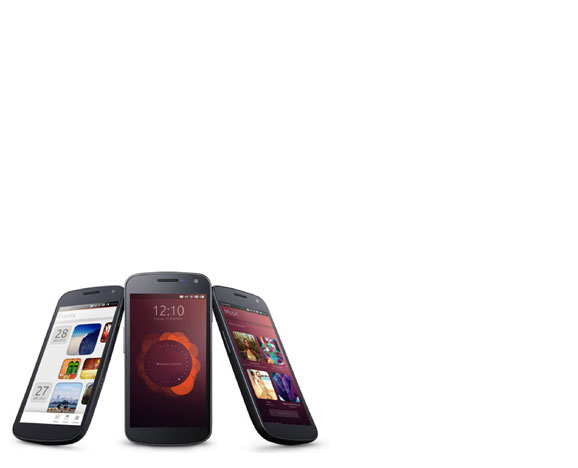
\includegraphics[width=0.7\linewidth]{/Users/Gianguido/Desktop/LinuxDayTalk/l1}
\end{center}
\end{frame}

\begin{frame}
\frametitle{Linux su smartphone... oggi!}
\begin{center}
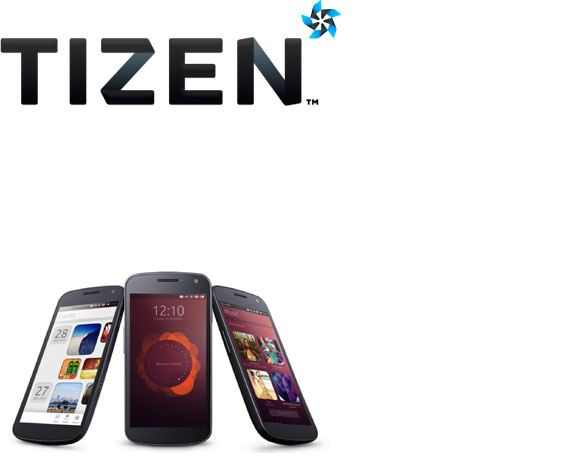
\includegraphics[width=0.7\linewidth]{/Users/Gianguido/Desktop/LinuxDayTalk/l2}
\end{center}
\end{frame}

\begin{frame}
\frametitle{Linux su smartphone... oggi!}
\begin{center}
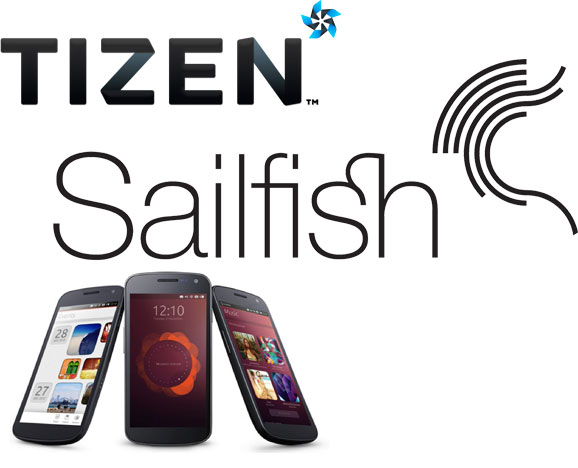
\includegraphics[width=0.7\linewidth]{/Users/Gianguido/Desktop/LinuxDayTalk/l3}
\end{center}
\end{frame}

\begin{frame}
\frametitle{Una panoramica su SalfishOS}
\begin{itemize}
\item SailfishOS è un sistema operativo basato su Mer e Nemo
\end{itemize}
\end{frame}

\begin{frame}
\frametitle{Una panoramica su SalfishOS}
\begin{itemize}
\item SailfishOS è un sistema operativo basato su Mer e Nemo
\item È sviluppato da una società finlandese chiamata Jolla
\end{itemize}
\end{frame}

\begin{frame}
\frametitle{Una panoramica su SalfishOS}
\begin{itemize}
\item SailfishOS è un sistema operativo basato su Mer e Nemo
\item È sviluppato da una società finlandese chiamata Jolla
\item È open-source al 90\%: alcuni componenti grafici verranno resi FOSS in futuro mentre i driver dovranno rimanere proprietari...
\end{itemize}
\end{frame}

\begin{frame}
\frametitle{Una panoramica su SalfishOS}
\begin{itemize}
\item SailfishOS è un sistema operativo basato su Mer e Nemo
\item È sviluppato da una società finlandese chiamata Jolla
\item È open-source al 90\%: alcuni componenti grafici verranno resi FOSS in futuro mentre i driver dovranno rimanere proprietari...
\item Utilizza tutte le nuove tecnologie disponibili in ambiente Linux:
\end{itemize}
\end{frame}

\begin{frame}
\frametitle{Una panoramica su SalfishOS}
\begin{itemize}
\item SailfishOS è un sistema operativo basato su Mer e Nemo
\item È sviluppato da una società finlandese chiamata Jolla
\item È open-source al 90\%: alcuni componenti grafici verranno resi FOSS in futuro mentre i driver dovranno rimanere proprietari...
\item Utilizza tutte le nuove tecnologie disponibili in ambiente Linux:
\begin{itemize}
\item Wayland
\end{itemize}
\end{itemize}
\end{frame}

\begin{frame}
\frametitle{Una panoramica su SalfishOS}
\begin{itemize}
\item SailfishOS è un sistema operativo basato su Mer e Nemo
\item È sviluppato da una società finlandese chiamata Jolla
\item È open-source al 90\%: alcuni componenti grafici verranno resi FOSS in futuro mentre i driver dovranno rimanere proprietari...
\item Utilizza tutte le nuove tecnologie disponibili in ambiente Linux:
\begin{itemize}
\item Wayland
\item PulseAudio
\end{itemize}
\end{itemize}
\end{frame}
\begin{frame}
\frametitle{Una panoramica su SalfishOS}
\begin{itemize}
\item SailfishOS è un sistema operativo basato su Mer e Nemo
\item È sviluppato da una società finlandese chiamata Jolla
\item È open-source al 90\%: alcuni componenti grafici verranno resi FOSS in futuro mentre i driver dovranno rimanere proprietari...
\item Utilizza tutte le nuove tecnologie disponibili in ambiente Linux:
\begin{itemize}
\item Wayland
\item PulseAudio
\item systemd
\end{itemize}
\end{itemize}
\end{frame}
\begin{frame}
\frametitle{Una panoramica su SalfishOS}
\begin{itemize}
\item SailfishOS è un sistema operativo basato su Mer e Nemo
\item È sviluppato da una società finlandese chiamata Jolla
\item È open-source al 90\%: alcuni componenti grafici verranno resi FOSS in futuro mentre i driver dovranno rimanere proprietari...
\item Utilizza tutte le nuove tecnologie disponibili in ambiente Linux:
\begin{itemize}
\item Wayland
\item PulseAudio
\item systemd
\item BTRFS
\end{itemize}
\end{itemize}
\end{frame}

\begin{frame}
\frametitle{Una panoramica su SalfishOS}
\begin{itemize}
\item SailfishOS è un sistema operativo basato su Mer e Nemo
\item È sviluppato da una società finlandese chiamata Jolla
\item È open-source al 90\%: alcuni componenti grafici verranno resi FOSS in futuro mentre i driver dovranno rimanere proprietari...
\item Utilizza tutte le nuove tecnologie disponibili in ambiente Linux:
\begin{itemize}
\item Wayland
\item PulseAudio
\item systemd
\item BTRFS
\item Qt 5, QML, QtQuick 2.0
\end{itemize}
\end{itemize}
\end{frame}


\begin{frame}
	\frametitle{Una panoramica su SalfishOS}
	\begin{itemize}
		\item Jolla vende l'unico dispositivo
	\end{itemize}
\end{frame}

\begin{frame}
	\frametitle{Una panoramica su SalfishOS}
	\begin{itemize}
		\item Jolla vende l'unico dispositivo
		\item Per natura aperta della società gli utenti possono collaborare a SailfishOS tramite http://together.jolla.com
	\end{itemize}
\end{frame}

\begin{frame}
	\frametitle{Una panoramica su SalfishOS}
	\begin{itemize}
		\item Jolla vende l'unico dispositivo
		\item Per natura aperta della società gli utenti possono collaborare a SailfishOS tramite http://together.jolla.com
		\item Per aiutare basta avere idee :-)
	\end{itemize}
\end{frame}


\begin{frame}
	\frametitle{Il punto di vista dell'utente}
	\begin{itemize}
		\item La UI/UX è stata concepita da 0, si basa su swipe
	\end{itemize}
\end{frame}

\begin{frame}
	\frametitle{Il punto di vista dell'utente}
	\begin{itemize}
		\item La UI/UX è stata concepita da 0, si basa su swipe
		\item Le applicazioni possono avvalersi di un background reale
	\end{itemize}
\end{frame}

\begin{frame}
	\frametitle{Il punto di vista dell'utente}
	\begin{itemize}
		\item La UI/UX è nuova, si basa su swipe
		\item Le applicazioni possono avvalersi di un background reale
		\item Lo store contiene già moltissime applicazioni utili, tra cui i maggiori social
	\end{itemize}
\end{frame}

\begin{frame}
	\frametitle{Il punto di vista dell'utente}
	\begin{itemize}
		\item La UI/UX è nuova, si basa su swipe
		\item Le applicazioni possono avvalersi di un background reale
		\item Lo store contiene già moltissime applicazioni utili, tra cui i maggiori social
		\item Sul device venduto da Jolla è disponibile un layer di compatibilità con app Android
	\end{itemize}
\end{frame}

\begin{frame}
	\frametitle{Il punto di vista dell'utente}
	\begin{itemize}
		\item La UI/UX è nuova, si basa su swipe
		\item Le applicazioni possono avvalersi di un background reale
		\item Lo store contiene già moltissime applicazioni utili, tra cui i maggiori social
		\item Sul device venduto da Jolla è disponibile un layer di compatibilità con app Android
		\item Il livello di privacy utente è alta
	\end{itemize}
\end{frame}

\begin{frame}
	\frametitle{Il punto di vista dell'hacker}
	\begin{itemize}
		\item I permessi di root sono facili da ottenere
	\end{itemize}
\end{frame}

\begin{frame}
	\frametitle{Il punto di vista dell'hacker}
	\begin{itemize}
		\item I permessi di root sono facili da ottenere
		\item I sorgenti del kernel e della parte FOSS del sistema sono sempre aggiornati e disponibili su GitHub
	\end{itemize}
\end{frame}


\begin{frame}
	\frametitle{Il punto di vista dell'hacker}
	\begin{itemize}
		\item I permessi di root sono facili da ottenere
		\item I sorgenti del kernel e della parte FOSS del sistema sono sempre aggiornati e disponibili su GitHub
		\item Il bootloader è facilmente sbloccabile
	\end{itemize}
\end{frame}

\begin{frame}
	\frametitle{Il punto di vista dell'hacker}
	\begin{itemize}
		\item I permessi di root sono facili da ottenere
		\item I sorgenti del kernel e della parte FOSS del sistema sono sempre aggiornati e disponibili su GitHub
		\item Il bootloader è facilmente sbloccabile
		\item Esiste uno store alternativo dove pubblicare le proprie creazioni
	\end{itemize}
\end{frame}

\begin{frame}
	\frametitle{Il punto di vista dell'hacker}
	\begin{itemize}
		\item I permessi di root sono facili da ottenere
		\item I sorgenti del kernel e della parte FOSS del sistema sono sempre aggiornati e disponibili su GitHub
		\item Il bootloader è facilmente sbloccabile
		\item Esiste uno store alternativo dove pubblicare le proprie creazioni
		\item C++, QT + QML per scrivere applicazioni
	\end{itemize}
\end{frame}

\begin{frame}
	\frametitle{Il punto di vista dell'hacker}
	\begin{itemize}
		\item I permessi di root sono facili da ottenere
		\item I sorgenti del kernel e della parte FOSS del sistema sono sempre aggiornati e disponibili su GitHub
		\item Il bootloader è facilmente sbloccabile
		\item Esiste uno store alternativo dove pubblicare le proprie creazioni
		\item C++, QT + QML per scrivere applicazioni
		\item Jolla incoraggia l'hacking dei propri dispositivi e di SailfishOS
	\end{itemize}
\end{frame}


\begin{frame}
\frametitle{La questione dei componenti interni}
\begin{itemize}
\item Android domani il mercato smartphone
\end{itemize}
\end{frame}

\begin{frame}
\frametitle{La questione dei componenti interni}
\begin{itemize}
\item Android domani il mercato smartphone
\item I produttori di SoC e componentistica varia non rilasciano i driver sotto licenze open-source
\end{itemize}
\end{frame}

\begin{frame}
\frametitle{La questione dei componenti interni}
\begin{itemize}
\item Android domani il mercato smartphone
\item I produttori di SoC e componentistica varia non rilasciano i driver sotto licenze open-source
\item I driver per Android funzionano solo sulla suddetta piattaforma
\end{itemize}
\end{frame}

\begin{frame}
\frametitle{La questione dei componenti interni}
\begin{itemize}
\item Android domani il mercato smartphone
\item I produttori di SoC e componentistica varia non rilasciano i driver sotto licenze open-source
\item I driver per Android funzionano solo sulla suddetta piattaforma
\item Portarli verso Linux (quello "vero") sarebbe un'operazione lunga e dispendiosa
\end{itemize}
\end{frame}

\begin{frame}
	\frametitle{SailfishOS Hardware Adaptation Kit}
	\begin{itemize}
		\item Grazie a libhybris portare SailfishOS su dispositivi Android è semplice
	\end{itemize}
\end{frame}

\begin{frame}
	\frametitle{SailfishOS Hardware Adaptation Kit}
	\begin{itemize}
		\item Grazie a libhybris portare SailfishOS su dispositivi Android è semplice
		\item L'unico requisito è avere a disposizione una build di CyanogenMod 10.1.x
	\end{itemize}
\end{frame}

\begin{frame}
	\frametitle{SailfishOS Hardware Adaptation Kit}
	\begin{itemize}
		\item Grazie a libhybris portare SailfishOS su dispositivi Android è semplice
		\item L'unico requisito è avere a disposizione una build di CyanogenMod 10.1.x appropriata
		\item Non c'è bisogno di riscrivere driver e per la maggioranza dei componenti nemmeno di configurare nulla
	\end{itemize}
\end{frame}

\begin{frame}
	\begin{center}
		\textbf{Fine}
	\end{center}
\end{frame}
\end{document}
